%-*-coding: utf-8;-*-
\documentclass[italian,a4paper]{scrartcl}
\usepackage{amsmath,amssymb,amsthm,thmtools}
\usepackage{eucal,babel,a4}
\usepackage[nochapters]{classicthesis}
\usepackage[utf8]{inputenc}
\usepackage{graphicx,caption,subcaption}

\captionsetup[subfigure]{labelformat=empty}

\newcommand{\RR}{{\mathbb R}}
\newcommand{\C}{{\mathcal C}}
\newcommand{\defeq}{=}
\DeclareMathOperator{\diag}{diag}


\def\Xint#1{\mathchoice
{\XXint\displaystyle\textstyle{#1}}%
{\XXint\textstyle\scriptstyle{#1}}%
{\XXint\scriptstyle\scriptscriptstyle{#1}}%
{\XXint\scriptscriptstyle\scriptscriptstyle{#1}}%
\!\int}
\def\XXint#1#2#3{{\setbox0=\hbox{$#1{#2#3}{\int}$ }
\vcenter{\hbox{$#2#3$ }}\kern-.6\wd0}}
\def\dashint{\Xint-}

\declaretheoremstyle[
spaceabove=6pt, spacebelow=6pt,
headfont=\normalfont\itshape,
notefont=\mdseries, notebraces={(}{)},
bodyfont=\normalfont,
postheadspace=1em,
qed=,
shaded={rulecolor=pink!30,rulewidth=1pt,bgcolor=pink!10}
]{mystyle}

\declaretheorem[numberwithin=section,name=Teorema]{theorem}
\declaretheorem[sibling=theorem,name=Lemma]{lemma}
\declaretheorem[style=mystyle,sibling=theorem,name=Esercizio]{exercise}
\declaretheorem[style=mystyle,sibling=theorem,name=Esempio]{example}


\title{Sistemi lineari omogenei di equazioni differenziali}
\author{E. Paolini}
\date{5 dicembre 2014}

\begin{document}
\maketitle

\section*{Esponenziale di matrici}
Sia $A$ una matrice quadrata $n\times n$. Definiamo la norma (norma
operatoriale) di $A$ come segue:
\[
  \Vert A \Vert = \sup_{\lvert v\rvert \le 1} \lvert Av\rvert
\]
dove $\lvert v\rvert = \sqrt{v_1^2+ \dots + v_n^2}$ è l'usuale norma del
vettore $v\in \RR^n$. Osserviamo che $v\mapsto Av$ è una funzione
continua e che $\{v\colon \lvert v\rvert \le 1\}$ è un insieme
compatto, dunque il $\sup$ nella definizione è in realtà un $\max$.

Per le proprietà del $\sup$ si ha:
\[
  |Av| \le \Vert A \Vert\, \lvert v \rvert
\qquad\text{e}\qquad
  \Vert A B \Vert \le \Vert A \Vert \, \Vert B \Vert.
\]
Dunque possiamo affermare il valore assoluto di ogni elemento di una
matrice si stima con la norma della matrice: $\lvert A_{ij}\rvert \le
\Vert A \Vert$, infatti:
\[
  \lvert A_{ij} \rvert = \lvert (A e_j)_i\lvert \le \lvert A e_j\rvert
  \le \Vert A \Vert
\]
(dove $e_j$ è il $j$-esimo vettore della base canonica di $\RR^n$).

Se $A_k$ è una successione di matrici, diremo che $A_k\to A$ se ogni
elemento della matrice $A_k$ converge al corrispondente elemento della
matrice $A$: $(A_k)_{ij} \to A_{ij}$. Questo corrisponde a considerare
la matrice $n\times n$ come un vettore dello spazio $\RR^{(n^2)}$.

Se $A(t)$ è una funzione a valori matrici (ovvero una matrice i cui
elementi sono funzioni di $t$), si potrà farne la derivata
come si fa per le funzioni vettoriali: $(A'(t))_{ij} = (A_{ij}(t))'$
cioè componente per componente. Le usuali regole per le derivate
valgono anche per le matrici, in particolare non è difficile
verificare (si espliciti la definizione del prodotto di matrici) che
\[
 (A(t)B(t))' = A'(t) B(t) + A(t) B'(t)
\]
dove, puntualizziamo, è importante mantenere i prodotti nell'ordine
giusto, in quanto il prodotto di matrici può non essere commutativo.

Se $A$ è una matrice quadrata, si definisce la matrice potenza $A^k$
per ogni $k$ naturale, mediante le proprietà
\[
  A^0 = I, \qquad A^{k+1} = A^kA.
\]
(se $A$ è invertibile si possono definire anche le potenze negative
$A^{-k}=(A^{-1})^k = (A^k)^{-1}$).

Definiamo allora la matrice esponenziale di $A$:
\[
  e^A = \sum_{k=0}^\infty \frac{A^k}{k!}.
\]
Per dare significato a questa definizione dobbiamo verificare che la
serie appena scritta sia convergente. Cioè dobbiamo verificare che per
ogni coppia di indici $ij$ sia convergente la serie numerica:
\[
 \sum_{k=0}^\infty \frac{(A^k)_{ij}}{k!}.
\]
Per quanto detto prima sappiamo che $\lvert(A^k)_{ij}\rvert \le \Vert
A ^k\Vert \le \Vert A \Vert^k$. Dunque la serie in questione è
assolutamente convergente in quanto il suo valore assoluto si stima
con la serie
\[
 \sum_{k=0}^\infty \frac{\Vert A\Vert^k}{k!} = e^{\Vert A\Vert}
\]
che è convergente. La definizione della matrice $e^A$ è dunque
ben posta e si ha
\[
 \Vert e^A\Vert \le e^{\Vert A \Vert}.
\]

\begin{theorem}[proprietà dell'esponenziale matrice]
Siano $A$ e $B$ matrici quadrate $n\times n$ e $t$ uno scalare.
Valgono le seguenti proprietà:
\begin{enumerate}
\item $e^0 = I$ (dove $0$ è la matrice nulla $n\times n$ ed $I$ è la
  matrice identità con le stesse dimensioni);
\item se $AB=BA$ allora $e^AB = Be^A$;
\item $(e^{tA})' = A e^{tA}$;
\item $e^{-A} = (e^A)^{-1}$ (in particolare la matrice esponenziale è
  sempre invertibile);
\item se $u(t)$ è una funzione a valori in $\RR^n$ che soddisfa
  l'equazione differenziale $u'(t) = Au(t)$ allora $u(t) = e^{tA} u(0)$;
\item se $AB=BA$ allora $e^{A+B} = e^A e^B$;
\item se $A$ è invertibile allora $e^{ABA^{-1}} = Ae^BA^{-1}$;
\item se $A$ è la matrice diagonale $A = \diag(\lambda_1, \dots, \lambda_n)$, allora $e^A$
 è pure una matrice diagonale con $e^A = \diag(e^{\lambda_1},\dots, e^{\lambda_n})$;
\item se $A$ è una matrice triangolare con la diagonale nulla (cioè
  $A_{ij}=0$ se $i\ge j$) allora $e^A = \sum_{k=0}^n \frac{A^k}{k!}$
  (basta sommare i primi $n+1$ termini);
\item se $B$ è una matrice triangolare (cioè $B_{ij}=0$ se $i > j$)
  allora $B = D + A$ con $D$ matrice diagonale e $A$ matrice
  triangolare con la diagonale nulla e quindi $e^B = e^De^A$ si può
  calcolare riconducendosi ai punti precedenti.
\end{enumerate}
\begin{proof}
1. Per quanto riguarda $e^0$ osserviamo che per definizione $0^0=I$
mentre $0^k=0$ se $k>0$. Dunque direttamente dalla definizion si
ottiene $e^0=I$.

2. Se $AB=BA$ osserviamo che sia ha anche $A^k B=B A^k$ (la matrice $B$
commuta con ogni fattore del prodotto $A^k$). Dunque:
\[
 \sum_{k=0}^N \frac{A^k}{k!} B = B \sum_{k=0}^N \frac{A^k}{k!}
\]
e passando al limite $N\to \infty$ si ottiene $e^A B = B e^A$.

3. Per calcolare la derivata di $e^{tA}$ vogliamo dimostrare che la serie
che definisce $e^{tA}$ converge totalmente quando $t$ varia in un
qualunque intervallo limitato. Poniamo allora $t\in [-M,M]$. Si ha:
\[
  \sup_{t\in[-M,M]}\frac{\Vert (tA)^k\Vert}{k!}
  = \sup_{t\in[-M,M]}\frac{\lvert t\rvert^k \Vert A^k\Vert}{k!}
  \le \frac{M^k\Vert A\Vert^k}{k!}
\]
la cui serie è convergente qualunque sia $M\in \RR$. Dunque la serie
che definisce $e^{tA}$ è una serie di funzioni continue e derivabili
che converge totalmente su ogni intervallo limitato. Possiamo quindi
derivare la serie termine a termine:
\[
(e^{tA})' = \sum_{k=0}^\infty \frac{((tA)^k)'}{k!}
 = \sum_{k=1}^\infty \frac{kt^{k-1} A^k}{k!}
 = A \sum_{k=1}^\infty \frac{t^{k-1}A^{k-1}}{(k-1)!}
 = A e^{tA}.
\]

4. Dimostriamo ora che $U(t) = e^{tA}e^{-tA}=I$ per ogni $t$. Si ha:
\[
 U'(t) = A e^{tA}e^{-tA} + e^{tA}(-A)e^{-tA}
       = A e^{tA}e^{-tA} - A e^{tA}e^{-tA} = 0
\]
($Ae^{tA} = e^{tA}A$ in quanto $A$ e $tA$ commutano).
Dunque $U'(t)=0$ cioè $U(t)$ è costante ovvero $U(t)=U(0)$. Ma $U(0)=I$
in quanto $e^0=I$ e quindi $U(t)=I$ per ogni $t$.

5. Prendiamo l'equazione $u' = Au$, moltiplicando a sinistra per $e^{-tA}$ l'equazione diventa
$e^{-tA} u' - e^{-tA} Au=0$ cioè $(e^{-tA} u)' = 0$. Questo significa
che la funzione $e^{-tA}u = c$ costante e moltiplicando a sinistra per
$e^{tA}$ si ottiene dunque $u = e^{tA}c$ come volevasi dimostrare.

6. Per dimostrare la proprietà $e^{A+B}=e^A e^B$ consideriamo la quantità
$U(t) = e^{-t(A+B)} e^{tA} e^{tB}$. Se dimostriamo che $U$ è costante,
visto che $u(0)=I$ si avrà anche $U(1)=I$ che è equivalente a quanto
vogliamo dimostrare. Dunque verifichiamo che la derivata è nulla,
sfruttando l'ipotesi $AB=BA$ che ci permette di far commutare i prodotti:
\begin{align*}
U'(t) & = -(A+B)e^{-t(A+B)} e^{tA} e^{tB} + e^{-t(A+B)}Ae^{tA}e^{tB} +
e^{-t(A+B)}e^{tA} B e^{tB} \\
& = [-(A+B) + A + B] U(t) = 0.
\end{align*}

7. Se $A$ è invertibile allora $(ABA^{-1})^k = ABA^{-1}ABA\dots ABA^{-1}
= AB^k A^{-1}$. Dunque nelle somme parziali della serie che definisce l'esponenziale
$e^{ABA^{-1}}$ si può raccogliere $A$ a sinistra e $A^{-1}$ a destra e
al centro rimane la serie che definisce $e^B$.

8. Se la matrice $A$ è diagonale con $A_{ii}=\lambda_i$ allora $A^k$
risulta essere una matrice diagonale con $(A^k)_{ii} =
\lambda_i^k$. Dunque nella definizione di esponenziale $e^A$ i termini
della serie sono tutte matrici diagonali, e sulla diagonale compare la
serie che definisce l'esponenziale $e^{\lambda_i}$.

9. Se $A$ è una matrice triangolare con $A_{ij}=0$ quando $i\ge j$, si
osserva che $A^2$ avrà degli zeri anche sopra la diagonale:
$(A^2)_{ij}=0$ quando $i+1\ge j$ (si applichi la definizione di
prodotto, riga per colonna). Nelle moltiplicazioni successive $A^3,
A^4,\dots$ si aggiungerà sempre una diagonale di zeri finché la matrice non
si annulla completamente $A^n=0$. Dunque la serie che definisce $e^A$
contiene solo un numero finito di termini (i primi $n+1$) e può essere
calcolata esplicitamente.

10. L'ultima proprietà è una osservazione che non richiede dimostrazione.
\end{proof}
\end{theorem}

\section{Classificazione delle soluzioni dei sistemi di due equazioni
  differenziali lineari del primo ordine a coefficienti costanti}

In questa sezione studieremo le soluzioni del sistema:
\[
\begin{cases}
 x' = a x + b y\\
 y' = c x + d y
\end{cases}
\]
dove $a,b,c,d\in \RR$ sono dei parametri fissati e le incognite sono
$x=x(t)$ e $y=y(t)$ due funzioni reali di variabile $t$ reale.

Considerando la matrice
\[
A = \begin{pmatrix}
a & b \\
c & d
\end{pmatrix}
\]
e ponendo $u = \begin{pmatrix}x\\y\end{pmatrix}$, il sistema può essere scritto in modo più
compatto:
\[
 u'(t) = A u(t).
\]
Sappiamo allora, dalle proprietà dell'esponenziale di matrice, che le
soluzioni di tale sistema si possono scrivere nella forma:
\[
 u(t) = e^{tA}c \qquad \text{con } c=\begin{pmatrix}c_1\\c_2\end{pmatrix}
\]
dove $c_1$ e $c_2$ sono costante arbitrarie. In particolare per $c_1=c_2=0$ si
ottiene sempre la soluzione costante $u(t)=0$. Questo viene chiamato un \emph{punto
  di equilibrio} del sistema, in quanto la soluzione mantiene per ogni
$t$ il valore del dato iniziale.
Saremo particolarmente interessati a
capire se le soluzioni che si ottengono prendendo un diverso dato iniziale
sono \emph{stabili},
cioè convergono al punto $(0,0)$ oppure sono \emph{instabili} e quindi
tendono ad andarsene all'infinito.

\emph{Caso 1.}
\marginpar{autovalori reali distinti}
La matrice $A$ ha due autovalori reali distinti: $\lambda$, $\mu$.
In questo caso la matrice è dunque diagonalizzabile e si potrà scrivere:
\[
  A = P \Delta P^{-1}
\]
con $\Delta$ matrice diagonale $\Delta = \diag(\lambda,\mu)$
 e $P$ matrice del cambio di base. Le colonne
della matrice $P$ saranno gli autovettori $v$, $w$ relativi agli
autovalori $\lambda$, $\mu$ infatti (indichiamo con $(v,w)$ la matrice con colonne $v$ e $w$):
\[
  A P = A (v, w) = (\lambda v, \mu w) = P \Delta.
\]

Dunque le soluzioni del sistema sono:
\[
  u(t) = e^{tA}c = e^{tP\Delta P^{-1}}c = P e^{t\Delta} P^{-1}c
  = P \diag(e^{t \lambda},e^{t \mu}) k
\]
dove $k=P^{-1}c$ è un nuovo vettore di costanti
arbitrarie. Scrivendo la soluzione nelle coordinate $X,Y$ della base $v,w$ si ha $u(t) = (x(t),y(t)) = P(X(t),Y(t))$
e quindi
\[
\begin{cases}
X(t) = k_1 e^{\lambda t} \\
Y(t) = k_2 e^{\mu t}.
\end{cases}
\]

La relazione tra le coordinate $X$ e $Y$ si può ottenere eliminando la
$t$ nelle equazioni precedenti. Ricavando $t$ dalla prima equazione e
sostituendo nella seconda si ottiene
\[
Y = k_2 \left(\frac{X}{k_1}\right)^{\frac{\mu}{\lambda}}
  = c X^{\frac \mu \lambda}.
\]
Dunque nel piano $X,Y$ le curve $(X(t),Y(t))$ hanno supporto contenuto
nel grafico delle potenze con esponente $\mu/\lambda$.

\begin{figure}
\centering
 \begin{subfigure}{5cm}
  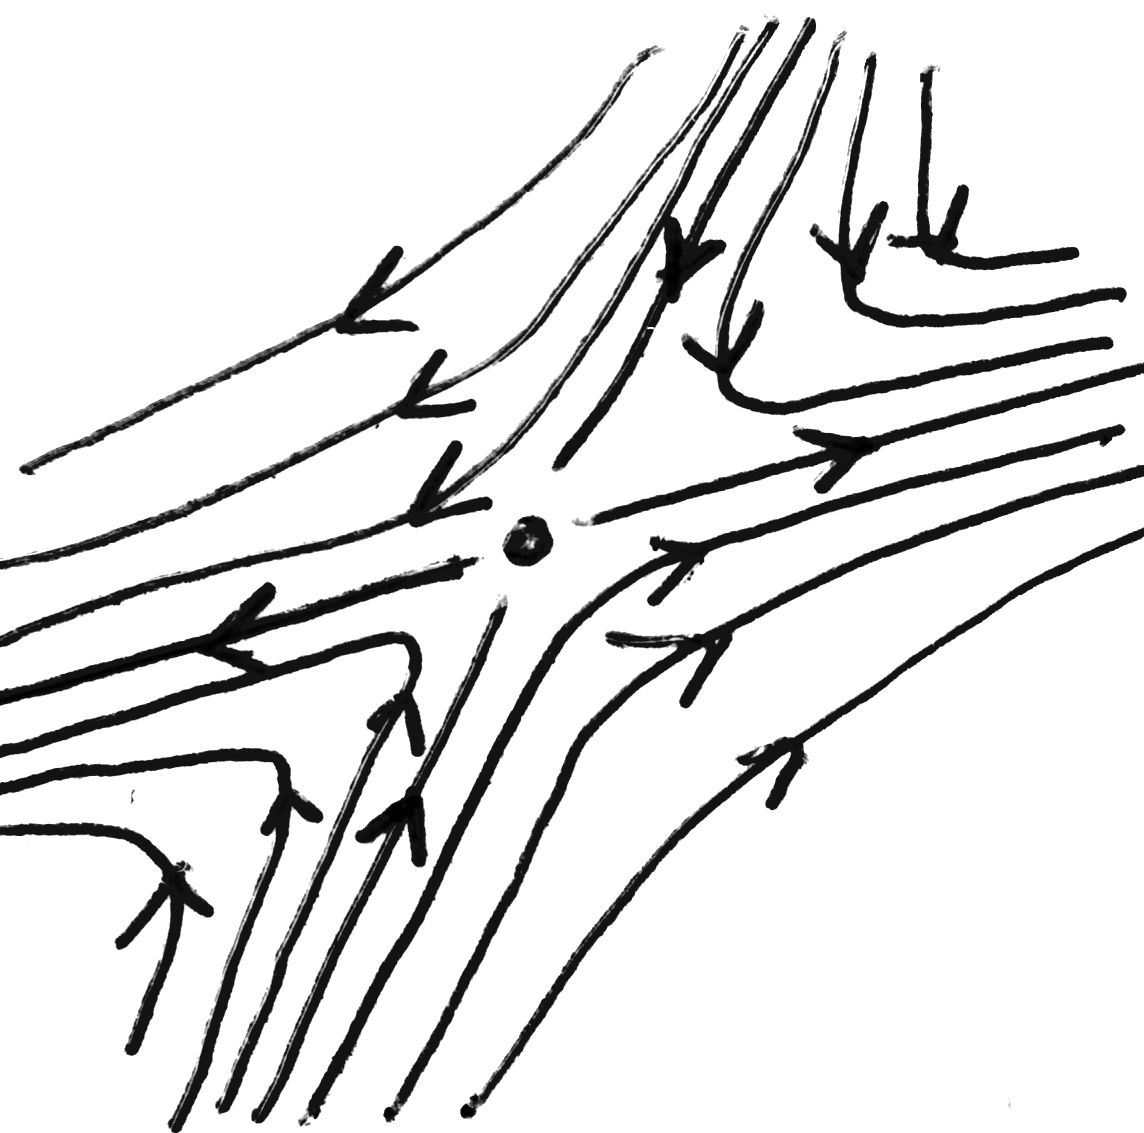
\includegraphics[width=0.75\textwidth]{sistemi_sella.png}
  \caption[1a]{sella (instabile)}
 \end{subfigure}
 \begin{subfigure}{5cm}
  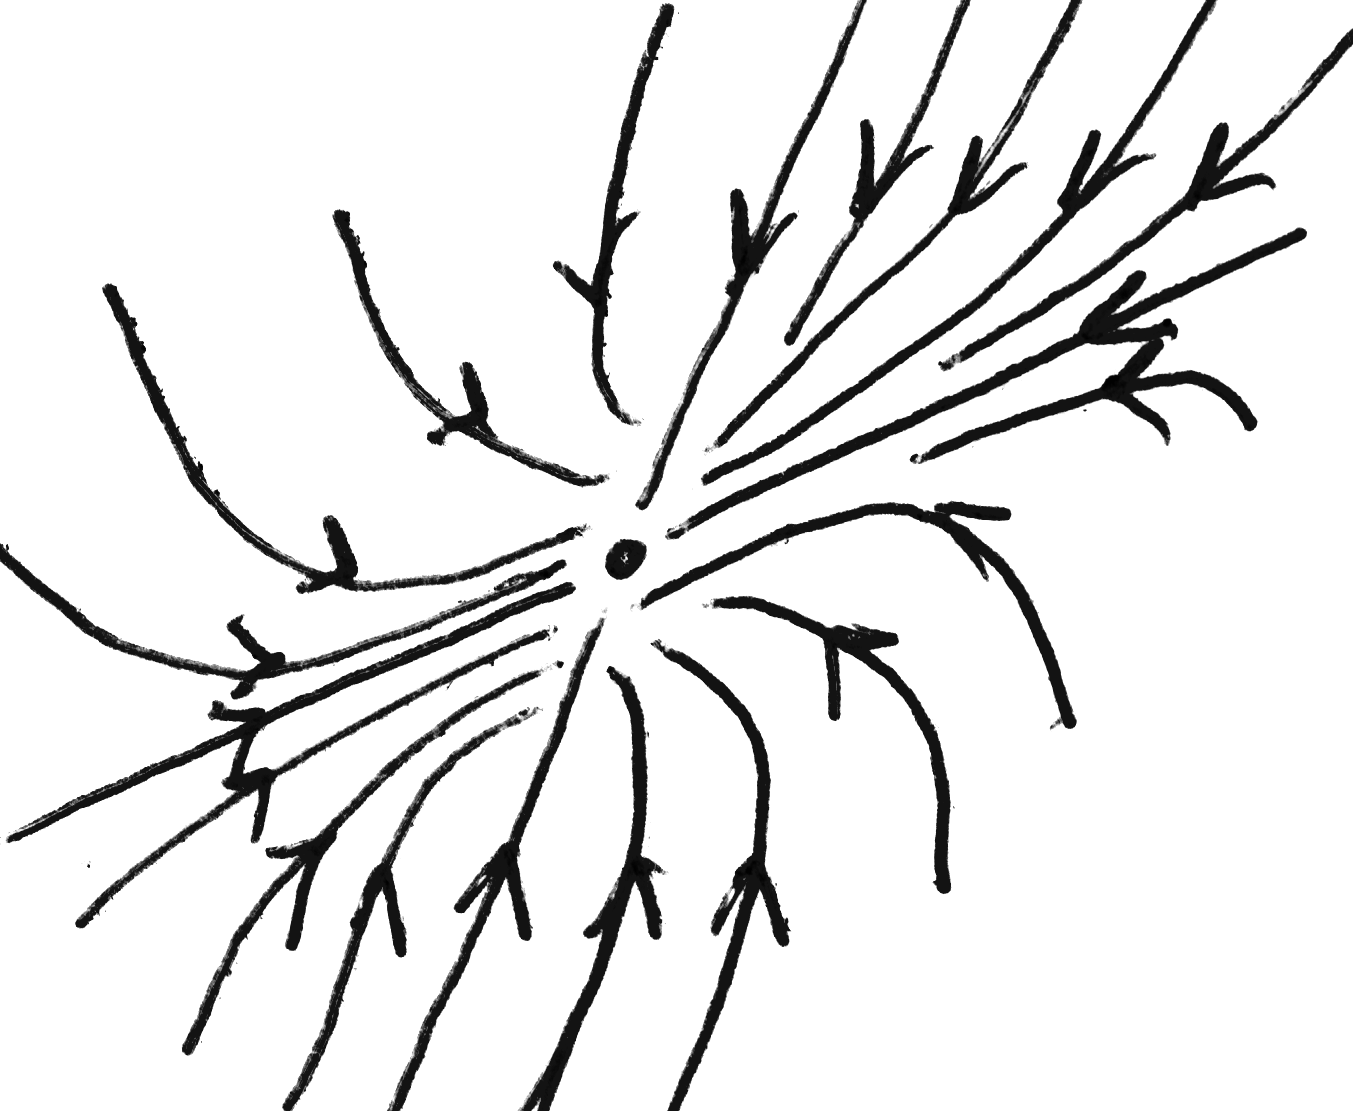
\includegraphics[width=0.75\textwidth]{sistemi_nodo.png}
  \caption{nodo stabile}
 \end{subfigure}
 \begin{subfigure}{5cm}
  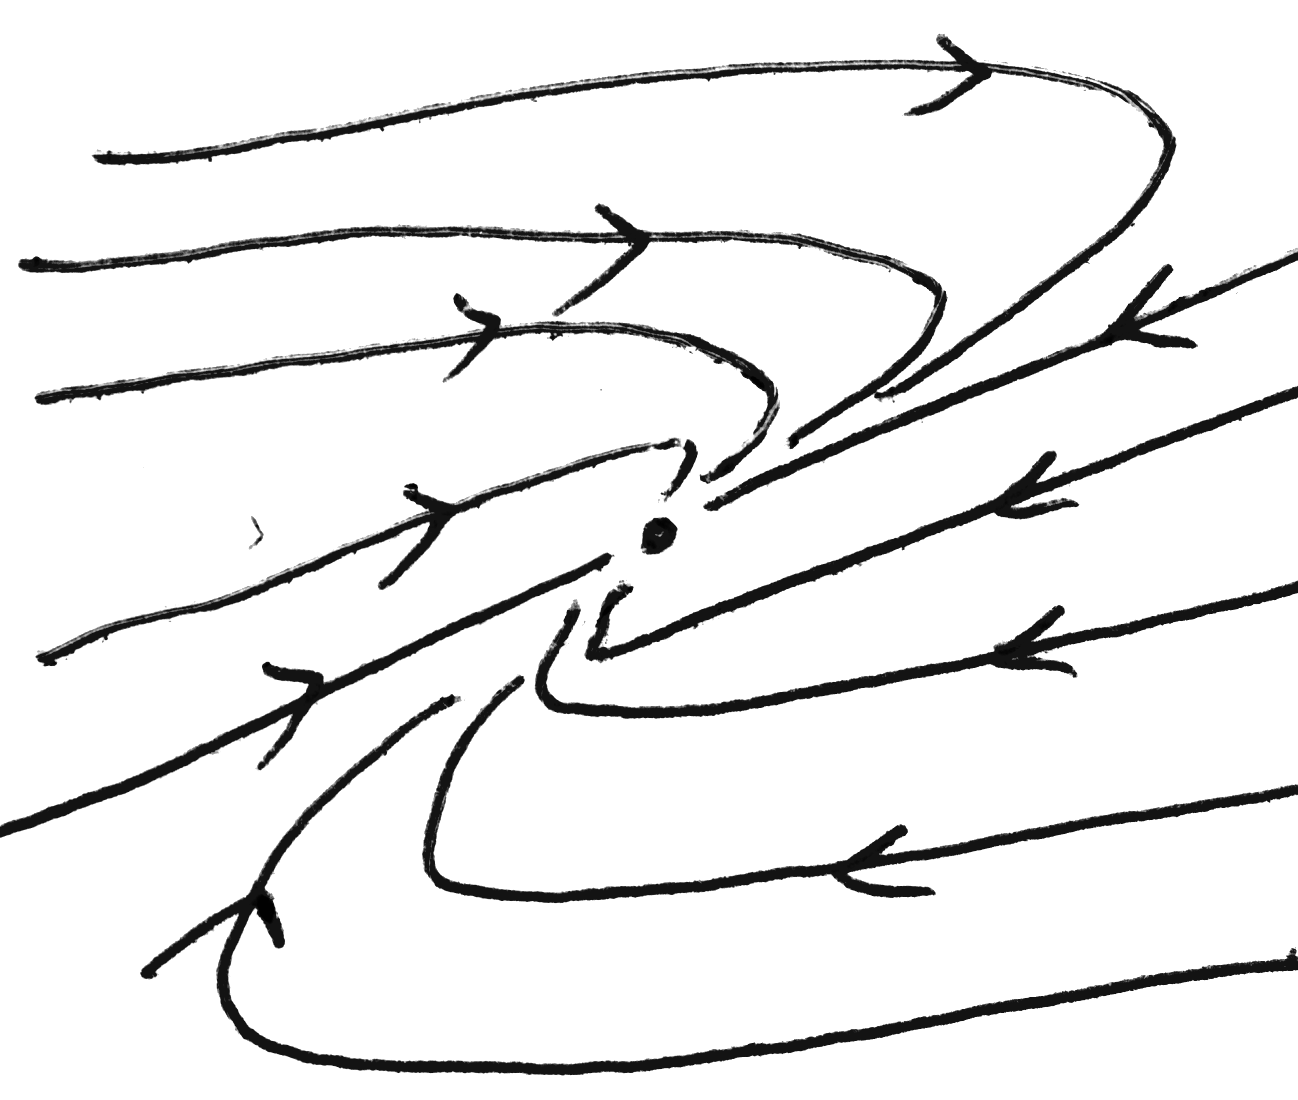
\includegraphics[width=0.75\textwidth]{sistemi_nodo_improprio.png}
  \caption{nodo improprio stabile}
 \end{subfigure}
 \begin{subfigure}{5cm}
  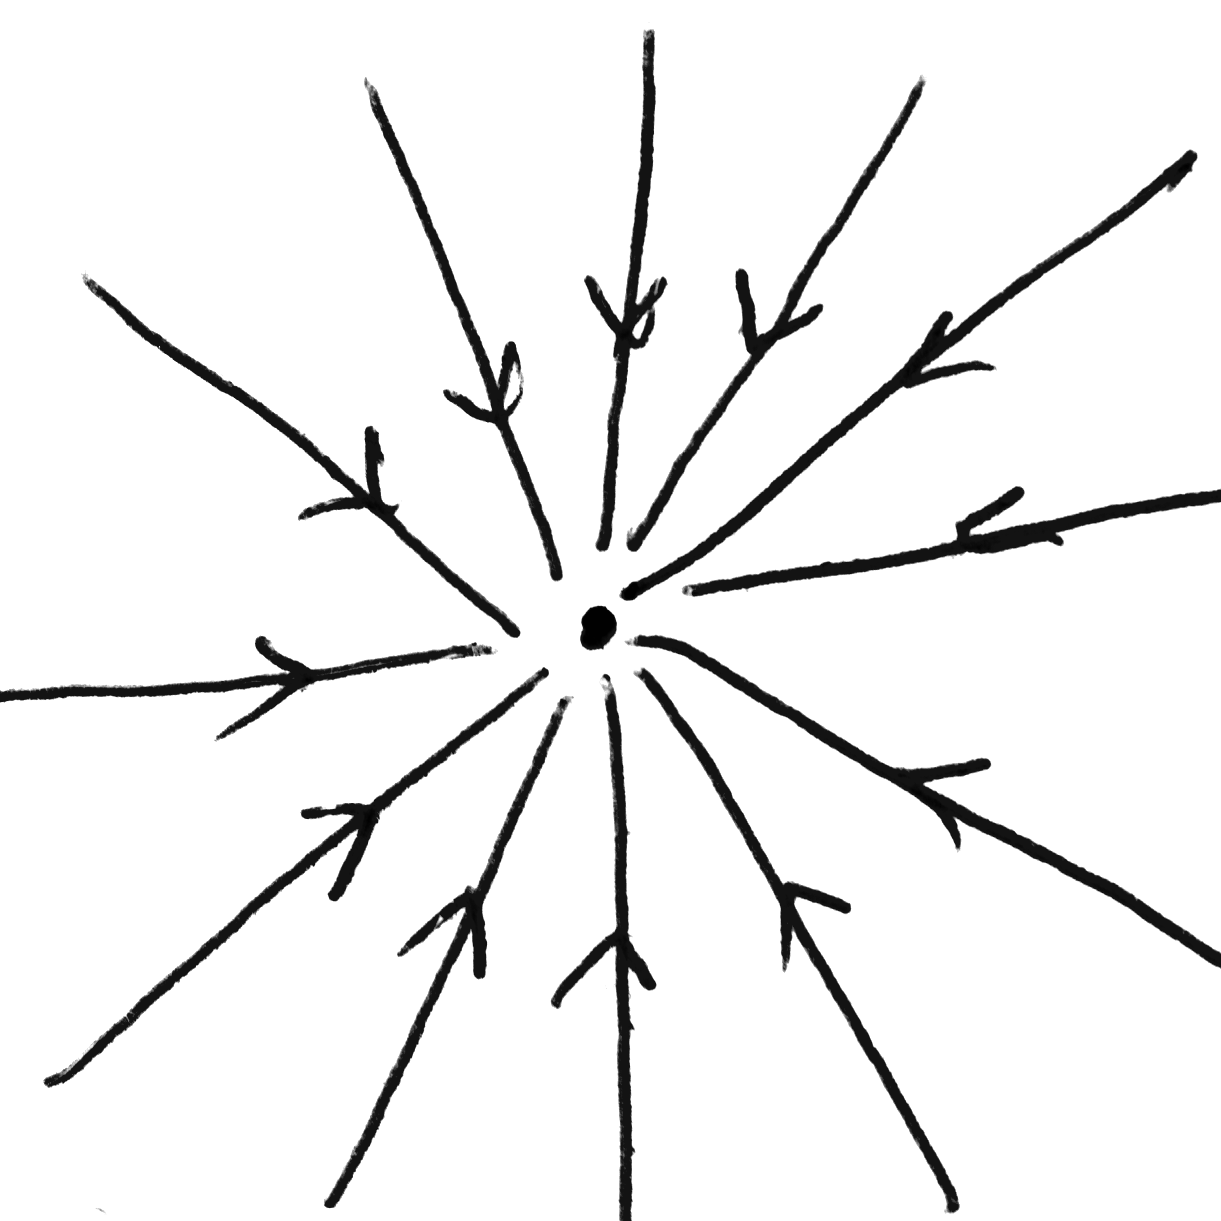
\includegraphics[width=0.75\textwidth]{sistemi_stella.png}
  \caption{stella stabile}
 \end{subfigure}
 \begin{subfigure}{5cm}
  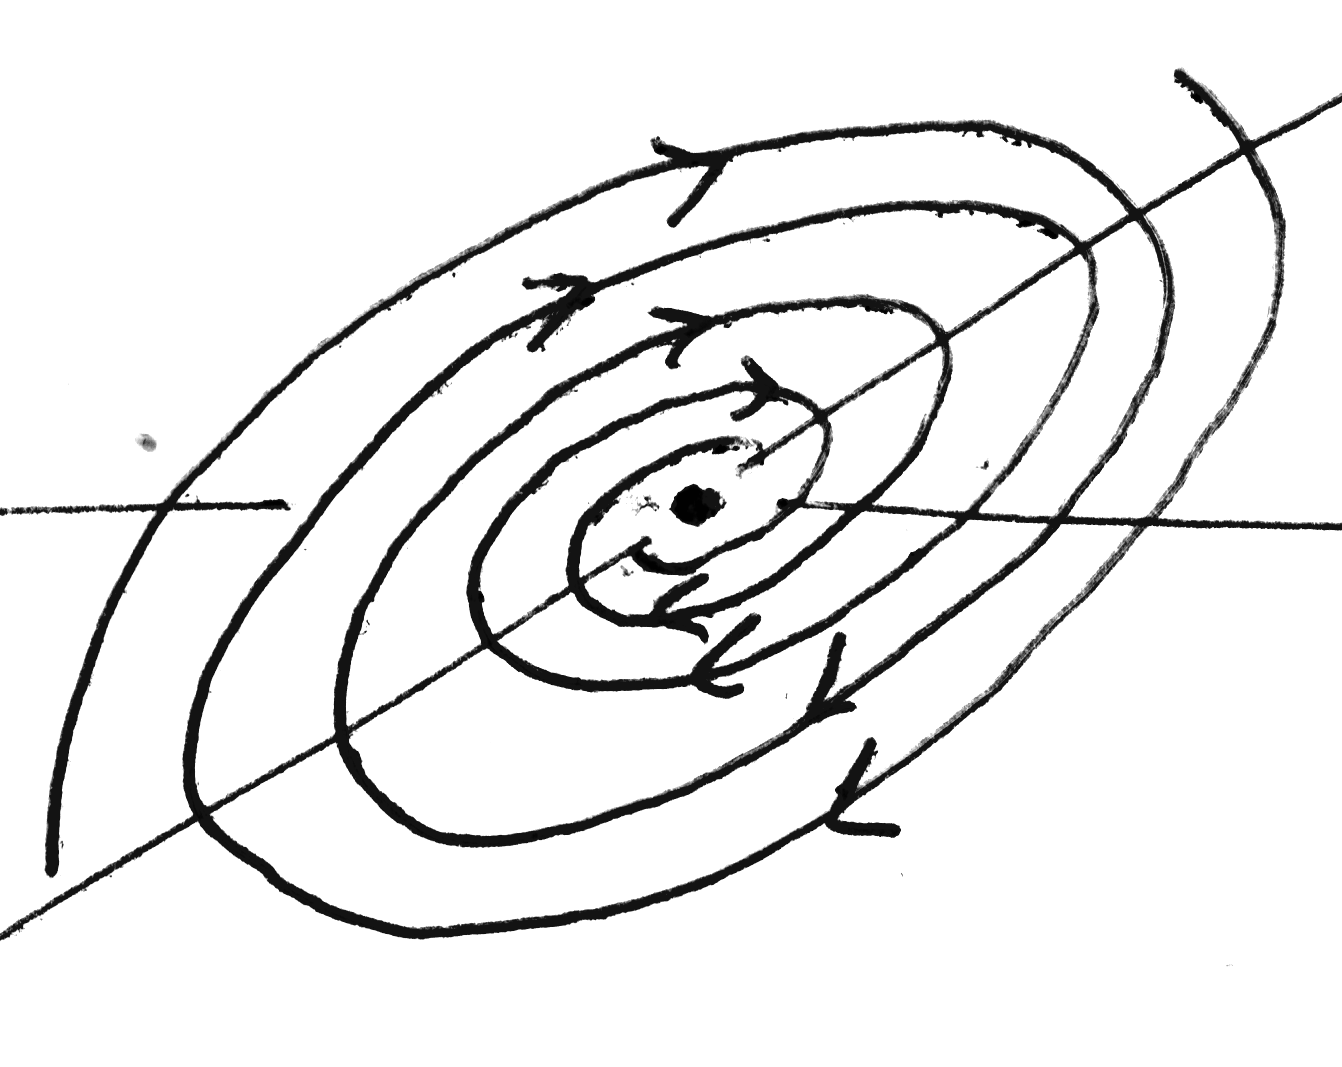
\includegraphics[width=0.75\textwidth]{sistemi_fuoco.png}
  \caption{fuoco stabile}
 \end{subfigure}
 \begin{subfigure}{5cm}
  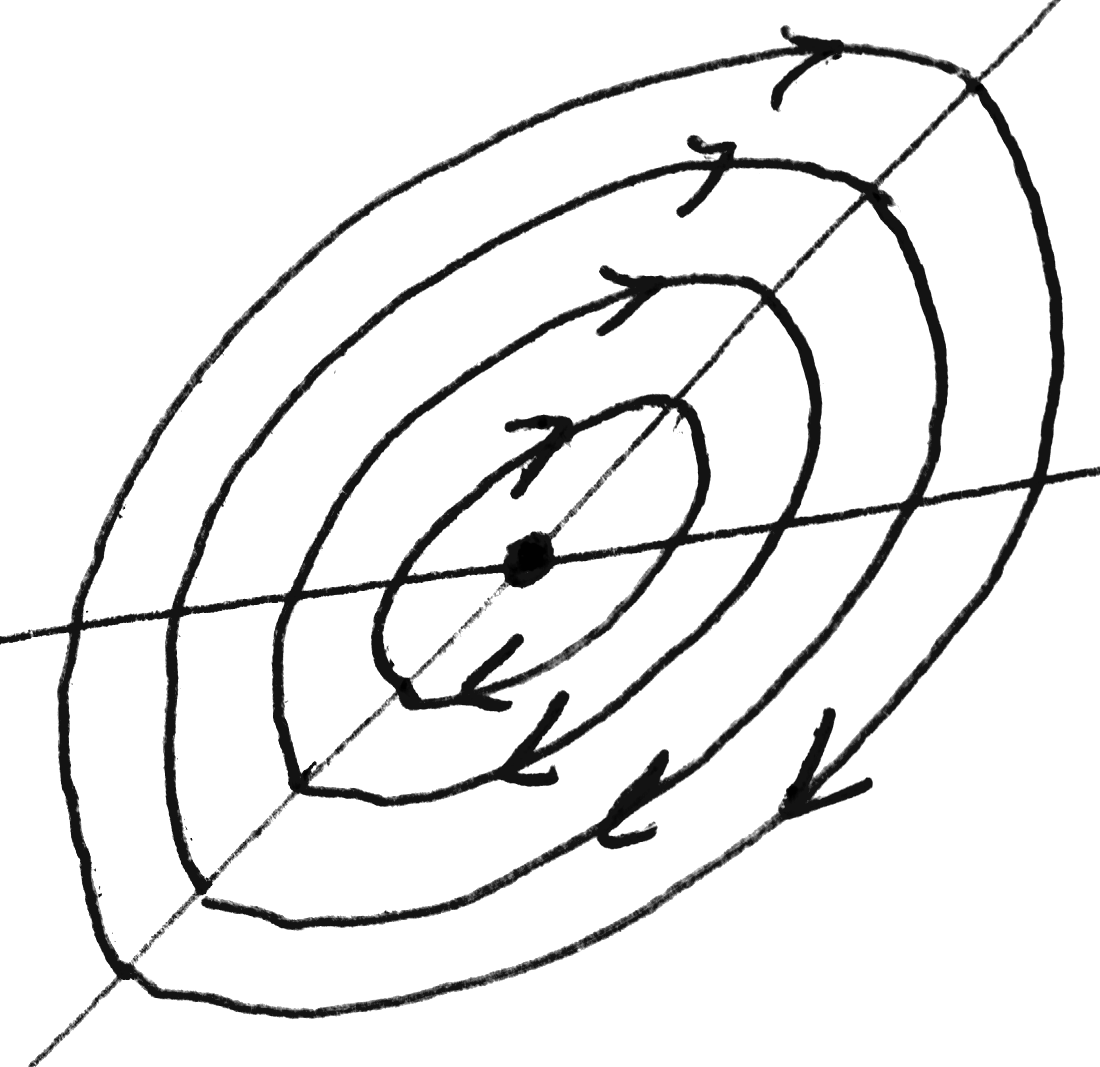
\includegraphics[width=0.75\textwidth]{sistemi_centro.png}
  \caption{centro (stabile)}
 \end{subfigure}
\end{figure}

\emph{Caso 1a.}
\marginpar{autovalori reali distinti di segno opposto, SELLA}
Se $\mu$ e $\lambda$ hanno segno opposto, allora
$\mu/\lambda<0$ e il grafico della potenze $X^{\mu/\lambda}$ ha
l'andamento di una iperbole (ma una vera iperbole si ottiene solamente
quando $\mu=-\lambda$).
Le soluzioni in questo caso sono dunque
instabili.
Si dice in questo caso che siamo di fronte ad un punto di \emph{sella}.

\emph{Caso 1b.}
\marginpar{autovalori reali distinti negativi, NODO STABILE}
Se $\mu$ e $\lambda$ sono entrambi negativi, allora il
grafico della potenza $X^{\mu/\lambda}$ ha l'andamento di una parabola
(ma una vera parabola si ottiene solamente quando $\mu=2\lambda$
oppure $\lambda=2 \mu$). Inoltre le curve sono orientate verso
l'origine (infatti le funzioni $X(t)=k_1 e^{\lambda t}$ e $Y(t)=k_2
e^{\mu t}$ tendono entrambe a zero per $t\to +\infty$). Si ha in
questo caso quello che viene chiamato un \emph{nodo asintoticamente
  stabile}.

\emph{Caso 1c.}
\marginpar{autovalori reali distinti positivi, NODO INSTABILE}
Se $\mu$ e $\lambda$ sono entrambi positivi, allora il
supporto delle curve soluzioni del sistema è lo stesso del caso
precedente. Ma l'orientazione è opposta, per $t\to \infty$ le
traiettorie si allontanano dall'origine e vanno all'infinito. Si parla
in questo caso di \emph{nodo instabile}.

\emph{Caso 2.}
\marginpar{matrice diagonale, STELLA}
Se la matrice $A$ è della forma
$\diag(\lambda,\lambda)=\lambda I$. Osserviamo che questo è equivalente a dire
 che $A$ ha un unico autovalore $\lambda$ con molteplicità algebrica 2 e
molteplicità geometrica 2 in quanto in tal caso l'autospazio
dell'autovettore $\lambda$ è l'intero spazio e in qualunque base la
matrice risulta essere diagonale.
Il sistema di equazioni differenziali è allora banale:
\[
\begin{cases}
 x' = \lambda x\\
 y' = \lambda y.
\end{cases}
\]
Le soluzioni sono tutte della forma: $x(t)=c_1 e^{\lambda t}$,
$y(t)=c_2 e^{\lambda t}$ le cui traiettorie hanno equazione
$y=\frac{c_2}{c_1}x$ cioè sono delle rette passanti per l'origine.
Se $\lambda<0$ le curve tendono asintoticamente all'origine $(0,0)$ e
si parla in questo caso di \emph{stella asintoticamente stabile}.
Se invece $\lambda>0$ si parla di \emph{stella instabile}. Se $\lambda
= 0$ tutte le soluzioni sono curve costanti, diremo quindi che le
soluzioni sono \emph{degeneri}.

\emph{Caso 3.}
\marginpar{autovalori coincidenti ma non diagonalizzabile, NODO IMPROPRIO}
Supponiamo che la matrice $A$ abbia un unico autovalore reale
$\lambda$ con molteplicità algebrica 2 ma supponiamo che la matrice
$A$ non sia diagonale. Sia $v$ un autovettore di $A$,
prendo un qualunque vettore $z$ indipendente da $v$ e considero
la base $v,z$. In questa base si ha $Av = \lambda v$, $Az = \alpha v +
\beta z$. Osserviamo che $\beta = \lambda$ in quanto il determinante
della matrice $A$ è $\lambda^2$ ed è invariante per cambio di
base, ma nella base $v,z$ la matrice che rappresenta $A$ è triangolare
ed ha $\lambda,\beta$ sulla diagonale.

Dunque $Az = \alpha v + \lambda z$. Ora sappiamo
che $\alpha\neq 0$ altrimenti $z$ sarebbe un secondo autovettore,
la molteplicità geometrica dell'autovalore $\lambda$ sarebbe $2$ e $A$
sarebbe diagonale. Dunque
prendiamo $w=z / \alpha$ e otteniamo $Av=\lambda v$, $Aw = v +
\lambda w$. Il vettore $w$ così trovato si chiama \emph{autovettore
  generalizzato} o \emph{pseudo-autovettore}. Ponendo $P=(v,w)$ (la
matrice del cambio di base, le cui colonne sono $v$ e $w$) si ha dunque:
\[
A = P B P^{-1}, \qquad B=\begin{pmatrix}\lambda & 1 \\ 0 & \lambda \end{pmatrix}
\]
e quindi le soluzioni sono:
\[
u(t) = e^{tA}c = P e^{tB}P^{-1}c = P e^{tB}k.
\]
con $k=P^{-1}c$.

La matrice $B$ viene chiamata \emph{forma canonica di Jordan} della matrice $A$.

Osserviamo ora che si può scrivere
\[
B = \lambda I + N \qquad\text{con}\qquad N=\begin{pmatrix}0&1\\0 & 0\end{pmatrix}.
\]
Da verifica diretta si trova $N^2=0$ e dunque $e^{tN} = I + tN$ (in base
all'ultima delle proprietà dell'esponenziale). Dunque
\begin{align*}
u(t) &= P e^{t\lambda I + tN}k = P e^{t\lambda I} (I + t N)k =
P e^{\lambda t} \begin{pmatrix} 1 & t \\ 0 & 1\end{pmatrix}\begin{pmatrix}k_1\\k_2\end{pmatrix}\\
& = P e^{\lambda t}\begin{pmatrix}k_1 + k_2 t \\ k_2\end{pmatrix}
\end{align*}
da cui, ponendo $u=(x,y) = P(X,Y)$, si trovano le soluzioni nella base
$v,w$:
\[
\begin{cases}
X(t) = (k_1 + k_2 t) e^{\lambda t}\\
Y(t) = k_2 e^{\lambda t}.
\end{cases}
\]
Se $\lambda<0$ le curve tendono all'origine quando $t\to +\infty$ e
abbiamo quindi un comportamento asintoticamente stabile. Se invece
$\lambda>0$ le curve tendono all'infinito e si ha dunque un
comportamento instabile.
Eliminando la $t$ ($t=\frac 1 \lambda \log\frac Y {k_2}$) e ponendo $a
= \frac{k_1}{k_2} - \frac{\log|k_2|}{\lambda}$ si ottiene
\[
X(t) = \left(a+\frac{\log|Y(t)|}{\lambda}\right)Y(t).
\]
Si vede che per $Y\to 0$ anche $X\to 0$ ma con pendenza $dx/dy$
infinita. Dunque le curve arrivano all'origine risultando tangenti
all'asse delle $X$. D'altra parte per $k_2=0$ si trovano delle
soluzioni con $Y=0$, dunque anche l'asse delle $x$ contiene soluzioni
dell'equazione.

Se $\lambda=0$ si ha una situazione degenere.

\emph{Caso 4.}
\marginpar{autovalori complessi coniugati}
Se la matrice $A$ è una matrice reale, (cioè coincide con la propria
coniugata: $\overline A=A$) con un autovalore complesso $\lambda =
\alpha + i\beta$, $\beta\neq 0$, con relativo autovettore complesso
$v+iw$, allora si ha
\[
  A(v+iw) = \lambda(v+iw)
\]
e quindi
\[
  A(v-iw) = \overline{A(v+iw)} = \overline{\lambda(v+iw)} = \bar \lambda (v-iw)
\]
che significa che $\overline \lambda = \alpha-i\beta$ è anch'esso un autovalore e $v-iw$ è l'autovettore associato. Dunque la matrice $A$ è diagonalizzabile nel campo complesso:
\[
  A = P D P^{-1},\qquad P=(v+iw, v-iw),\qquad D = \diag(\alpha+i\beta, \alpha-i\beta)
\]
($P$ è la matrice che ha come colonne i vettori complessi $v+iw$ e
$v-iw$).

Essendo $v+iw$ e $v-iw$ vettori complessi indipendenti, si può
facilmente mostrare che anche i vettori reali $v,w$ risultano essere
indipendenti. Osserviamo allora che
\[
 P = (v+iw, v-iw) = (v,w)\begin{pmatrix}1 & 1\\ i & -i\end{pmatrix}
\]
e che
\[
  P^{-1} = \begin{pmatrix}1 & 1\\ i & -1\end{pmatrix}^{-1}(v,w)^{-1}
         = \frac 1 2 \begin{pmatrix}1 & -i\\ 1 & i\end{pmatrix}(v,w)^{-1}
\]
e quindi nella base $v,w$ la matrice $A$ diventa:
\begin{align*}
\frac 1 2
\begin{pmatrix}1 & 1\\ i & -i\end{pmatrix}
\begin{pmatrix}\lambda & 0 \\ 0 & \bar \lambda\end{pmatrix}
\begin{pmatrix}1 & -i\\ 1 & i\end{pmatrix}
&=
\frac 1 2
\begin{pmatrix}\alpha+i\beta & \alpha-i\beta \\i\alpha-\beta  &
  -i\alpha-\beta\end{pmatrix}
\begin{pmatrix}1 & -i\\ 1 & i\end{pmatrix}\\
&=
\begin{pmatrix}\alpha & \beta \\-\beta  & \alpha\end{pmatrix}.
\end{align*}

Osserviamo qui che la matrice $A$ è diagonalizzabile in campo
complesso, ma non in campo reale. Una rappresentazione \emph{canonica}
di $A$ nel campo reale è quella data qui sopra, e viene chiamata
\emph{forma canonica reale di Jordan}. I vettori $v,w$ che sono parte reale
e parte immaginaria degli autovettori complessi di $A$, possono anche
essere identificati dalle seguenti proprietà:
\[
  Av = \alpha v - \beta w,\qquad Aw = \beta v + \alpha w.
\]

Le soluzioni del sistema sono dunque, al variare di $c\in \RR^2$:
\begin{align*}
u(t) & = e^{tA} c = P e^{tD}P^{-1} c
       = P e^{tD} \frac 1 2 \begin{pmatrix}1 & -i\\ 1 & i\end{pmatrix} k
\end{align*}
dove si è posto $k=(v,w)^{-1} c$. Dunque
\begin{align*}
  u(t) &= \frac 1 2 P \begin{pmatrix}e^{\lambda t} & 0 \\ 0 & e^{\bar \lambda t}\end{pmatrix}
          \begin{pmatrix}k_1 - ik_2\\ k_1 + i k_2\end{pmatrix}\\
 &= \frac 1 2 P \begin{pmatrix}e^{\alpha t + i \beta t}(k_1-ik_2) \\ e^{\alpha t - i \beta t}(k_1 + i k_2)\end{pmatrix} \\
 &= \frac 1 2 P e^{\alpha t}\begin{pmatrix} e^{i\beta t}(k_1-ik_2) \\
  e^{-i\beta t}(k_1 + ik_2)\end{pmatrix}.
\end{align*}
Scrivendo il numero complesso $k_1 + i k_2$ in coordinate polari si potranno trovare $\rho$ e $\phi$ tali
che $k_1 + i k_2 = \rho e^{-i\phi}$. Si avrà allora
\begin{align*}
u(t)
&=
\frac 1 2 \rho e^{\alpha t}P\begin{pmatrix}
e^{i\beta t} e^{i\phi} \\
e^{-i\beta t} e^{-i\phi}
\end{pmatrix}\\
&=
\frac 1 2 \rho e^{\alpha t} (v,w)
\begin{pmatrix}1 & 1 \\ i & -i\end{pmatrix}
\begin{pmatrix}
e^{i(\beta t+\phi)} \\
e^{-i(\beta t+\phi)}
\end{pmatrix}\\
& =
\frac 1 2 (v,w) \rho e^{\alpha t}
\begin{pmatrix}
e^{i(\beta t+\phi)} + e^{-i(\beta t+\phi)}\\
ie^{i(\beta t+\phi)} - ie^{-i(\beta t+\phi)}
\end{pmatrix}\\
&=
(v,w)
\begin{pmatrix}
\rho e^{\alpha t}
\cos(\beta t+\phi))\\
-\rho e^{\alpha t}
\sin(\beta t+\phi))
\end{pmatrix}
\end{align*}
da cui, se $X,Y$ sono le coordinate di $u(t)$ nella base $v,-w$, si ha
\begin{align*}
X(t) &= \rho e^{\alpha t} \cos(\beta t+\phi))\\
Y(t) &= \rho e^{\alpha t} \sin(\beta t+\phi)),
\end{align*}
dove, ricordiamo, $\alpha$ e $\beta$ sono parte reale e parte
immaginaria del primo autovalore complesso, mentre $\rho\ge 0$ e $\phi\in[0,2\pi)$
(ampiezza e fase) sono parametri arbitrari ognuno dei quali ci
fornisce una diversa soluzione.

Se $\alpha=0$
\marginpar{CENTRO (stabile)}
(cioè i due autovalori di $A$ sono immaginari puri)
allora le soluzioni descrivono nel piano $X,Y$ dei cerchi concentrici
centrati nell'origine. Nel piano $x,y$ saranno dunque delle ellissi
con gli assi paralleli ai vettori $v$ e $w$. Questa configurazione si
chiama \emph{centro} ed è una configurazione \emph{stabile} (ma non
asintoticamente)
nel senso che le traiettorie rimangono limitate, pur non convergendo
all'origine.

Se $\alpha<0$
\marginpar{FUOCO asintoticamente stabile}
le traiettorie descrivono delle spirali logaritmiche che convergono
verso l'origine. Il verso di rotazione è da $w$ verso $v$ se $\beta$ è
positivo, da $v$ verso $w$ se $\beta$ è negativo.
Si dice allora che siamo in presenza di un
\emph{fuoco asintoticamente stabile}.

Se $\alpha>0$
\marginpar{FUOCO instabile}
le traiettorie descrivono delle spirali che si allontanano
dall'origine divergendo all'infinito. Il senso di rotazione è
determinato da $\beta$ come nel caso precedente.
Questa configurazione è chiamata \emph{fuoco asintoticamente instabile}.

\section*{Aggiornamenti}
\begin{itemize}
\item[13.12.2014] aggiunte figure e revisione generale.
\item[12.9.2015] piccoli aggiustamenti.
\end{itemize}
\end{document}
